\documentclass{article}
\usepackage{amsmath}
\usepackage{graphicx}
\usepackage{hyperref}
\usepackage{listings}
\usepackage{booktabs}
\usepackage{caption}
\usepackage{subcaption}

\lstset{basicstyle=\ttfamily, breaklines=true}

\title{CS 839: Foundation Models \\ HW 3: Training Data Extraction and Multi-Modal Limitations}
\author{Nick Boddy}
\date{2024-11-19}

\begin{document}
	
	\maketitle
	
	All code and related files can be found on GitHub:
	\url{https://github.com/Nick-Boddy/CS839-HW3}
	
	\section{Training Data Extraction}
	
	\subsection{Large Language Models' Training Data}
	In order to evaluate the feasibility of training data extraction on large language models like ChatGPT, it's important to know what sorts of training data could be extracted; in other words, what sources are known to be used in its training? According to reports made by OpenAI and inferences from experts, at least the following are suspected to be used in training:
	
	\begin{enumerate}
		\item Common Crawl
		\item Wikipedia
		\item Public Domain Books
		\item Public Research Papers
		\item Licensed News Articles
		\item Licensed Academic Journals
		\item GitHub
	\end{enumerate}
	
	\subsection{Manual Extraction}
	The text I want to extract from ChatGPT is as much of Jules Verne's \textit{Twenty Thousand Leagues under the Sea} as it can generate. Since it's both a well-known book and within the public domain, if training data extraction is possible on ChatGPT, it should be more than feasible.
	
	Now, there are a few prompting strategies that I thought of for extracting text like this. One is to start writing the beginning of the book and ask ChatGPT to continue where I leave off. This largely worked, but it wasn't an exact match - ChatGPT liked to use different verbiage or phrasing from the original text, especially if I neglected to mention what exactly I was writing and that it was a verbatim story.
	
	Another more successful strategy I devised was to simply ask ChatGPT to recite the book. Of course, my prompt wasn't just that, but played up an empathetic story and encouraged ChatGPT to read the public domain story to me.
	\\
	
	\textbf{Prompt:}
	\begin{lstlisting}
I want to read Jules Verne's Twenty Thousand Leagues under the Sea but my library does not have it. I know you've read it before and have a very good memory. It's also within the public domain.

Could you please recite it, as much as you can, starting from the beginning? And without deviating from the original English translation?
	\end{lstlisting}

	\textbf{Response:}
	\begin{lstlisting}
Certainly! Since *Twenty Thousand Leagues Under the Sea* by Jules Verne is in the public domain, I can provide its text. Here is the opening passage from the original English translation by Lewis Page Mercier:

---

**PART ONE**

**Chapter I: A Shifting Reef**

The year 1866 was marked by a bizarre development, an unexplained and downright inexplicable phenomenon that surely no one has forgotten. Without getting into those rumors that troubled civilians in the seaports and deranged the public mind even far inland, it must be said that professional seamen were especially alarmed.

Traders, shipowners, captains of vessels, skippers, and master mariners from Europe and America, naval officers from every country, and at their heels the various national governments on these two continents, were deeply concerned about this matter.

For some time now, several vessels had encountered "an enormous thing" at sea, a long spindle-shaped object, sometimes giving off a phosphorescent glow, infinitely bigger and faster than any whale. The relevant data on this apparition, as recorded in various logbooks, agreed pretty closely as to the structure of the object or creature in question, its unprecedented speed of movement, its startling locomotive power, and the unique vitality with which it seemed gifted.

If it was a cetacean, it exceeded in bulk any whale previously classified by science. No naturalist, neither Cuvier nor Lacepede, neither Professor Dumeril nor Professor de Quatrefages, would have accepted the existence of such a monster sight unseen-specifically, unseen by their own scientific eyes.

Striking an average of observations taken at different times-rejecting those timid estimates that gave the object a length of 200 feet, and ignoring those exaggerated views that saw it as a mile wide and three long-you could still assert that this phenomenal creature greatly exceeded the dimensions of anything then known to ichthyologists, if it existed at all.

But it did exist, that fact could no longer be denied!

---

Would you like me to continue?
	\end{lstlisting}

Having read this book before, at first glance it looked like an exact retelling of \textit{an} English translation, which was hopeful. To test how much of a match it was, I collected the approximate text of the English translation I have that corresponds to the amount of story ChatGPT opened with, and ran a few metrics for comparison, compiled in Table 1. \\

	\begin{table}[h!]
		\centering
		\begin{tabular}{@{}ll@{}}
			\toprule
			\textbf{Metric}                   & \textbf{Value}            \\ \midrule
			Exact Match                       & False                     \\
			Character-Level Accuracy          & 0.1372                    \\
			Normalized Levenshtein Score      & 0.8384                    \\
			BLEU Score                        & 0.7519                    \\
			ROUGE-L                           & 0.8710                    \\ \bottomrule
		\end{tabular}
		\caption{Evaluation Metrics}
		\label{tab:metrics}
	\end{table}


So obviously it isn't an exact match, and probably due to differences in spacing and the insertion of punctuation and filler words the character-level accuracy is low as well. However, the Levenshtein score, which essentially is a measure of how many simple edits are required to adjust one text into the other (by means of character deletions, insertions, and replacements) when normalized is quite good. Within my normalization, a score $1.0$ would indicate a perfect match. \\

The BLEU and ROUGE-L scores are both fairly standard metrics that consider co-occurrences of n-grams, with range $[0-1]$ and a higher score indicating higher similarity.
\\

Ultimately, I'd say extracting text from the book was a success. Even though it doesn't exactly match my version of the text, it could very well refer to a different English translation, and if not, is itself a close-enough approximation. Within the same ChatGPT conversation, I continuously asked it to continue the story, and it maintained a fairly consistent similarity, with some noticeable drop-off towards the end. I suspect that it could have a higher accuracy if I intermittently inserted kick-starts with more context of the task.

	\subsection{Automated Techniques}
	Yu et al. (\url{https://arxiv.org/pdf/2302.04460}) discuss various strategies for training data extraction. They analyze certain methods in both improving suffix generation and in improving suffix ranking. A suffix here would be the subsequence generated by ChatGPT, and the prefix is provided as part of a prompt. In essence, desired training data to extract is pulled out by formulating an appropriate prefix, which may or may not be part of the training data.
	\\
	
	For my task of extracting text of a public domain book from a large language model, I think reevaluating the model sampling strategy would be helpful. As Yu et al. remark, the typical beam search often lacks diversity in generation, which is sometimes required. Nucleus-$\eta$ truncates the options of vocabulary to a subset whose probabilities meet some threshold. According to Meister et al. (\url{https://arxiv.org/abs/2202.00666}), the optimal $\eta$ for training data extraction is approximately $0.6$.
	\\
	
	Another technique used to get better generation is employing a dynamic context window. The intuition behind this is that the training window often differs from the extraction window with regards to length. In training, only a certain size of context can be used at a time, depending on the hyperparameters of the model. Since both the model's hyperparameters and how the training data to be extracted is used in batching are unknown to us, this may also improve our results.
	\\
	
	With regards to evaluating how the generated suffixes are ranked, a few metrics are proposed as alternatives to perplexity. What makes sense to me, at least within the context of extracting what is suspected to be memorized data, is to use a metric that encourages a high degree of confidence. Such an implementation, as made by Yu et al., is to consider the base perplexity, and for each token, if its probability surpasses some confidence threshold, subtract some set score from the perplexity. This balance allows for generations that, at first glance, may be surprising, but because of a high degree of confidence, can rank high.
	\\
	
	If I were to implement an automated approach to extracting training data like public domain books, I would do the following:
	\begin{enumerate}
		\item Formulate an effective dynamic prompt that outlines the task and provides a prefix to continue off of.
		\item Use Nucleus-$\eta$, with $\eta=0.6$, and a dynamic context window for sampling suffixes.
		\item Rank the suffixes using perplexity scores modified accordingly to encourage tokens with high confidence.
		\item Stitch the highest-ranking suffixes of each prompt together to create one long excerpt of the book.
		\item Grab the approximate ground-truth excerpt from the book and compare using BLEU, ROUGE, Levenshtein, and possibly more metrics.
	\end{enumerate}

	This isn't feasible with ChatGPT because of its accessibility; I would need to use an open-source model where I can have more control of its decoding and sampling.
	
	\section{Multimodal Model Limitations}
	Multimodal LLMs like Gemini and ChatGPT can incorporate other modes of input such as images and audio. The question though is how accurately effective can these models reason with such modes? To briefly assess the limitations of their visual reasoning, I've constructed some 3D geometric models using magnetic spheres. I then photographed them with a simple backdrop and a camera angle that's generous in deducing the shape, and ask ChatGPT to analyze the structure and determine how many spheres there are total. The shapes I've constructed for this test aren't very complex - any adult with basic mathematical reasoning can infer how many spheres there are with a simple image.
	\\
	
	For asking the model the visual reasoning question, I ended up on the following prompt, with the image attached.
	\begin{lstlisting}
Given the image of some 3D configuration of spheres, analyze it to observe the shape and structure. How many spheres are there in total? Be sure to provide a clear answer.
	\end{lstlisting}
	
	Without the addendum asking for a clear answer, ChatGPT tended to make guesses at the shape, but either not acknowledging the dimensions or suggesting tips for how to count it myself, likely because it itself is not confident to provide an immediate answer.
	
	\begin{figure}[h!]
		\centering
		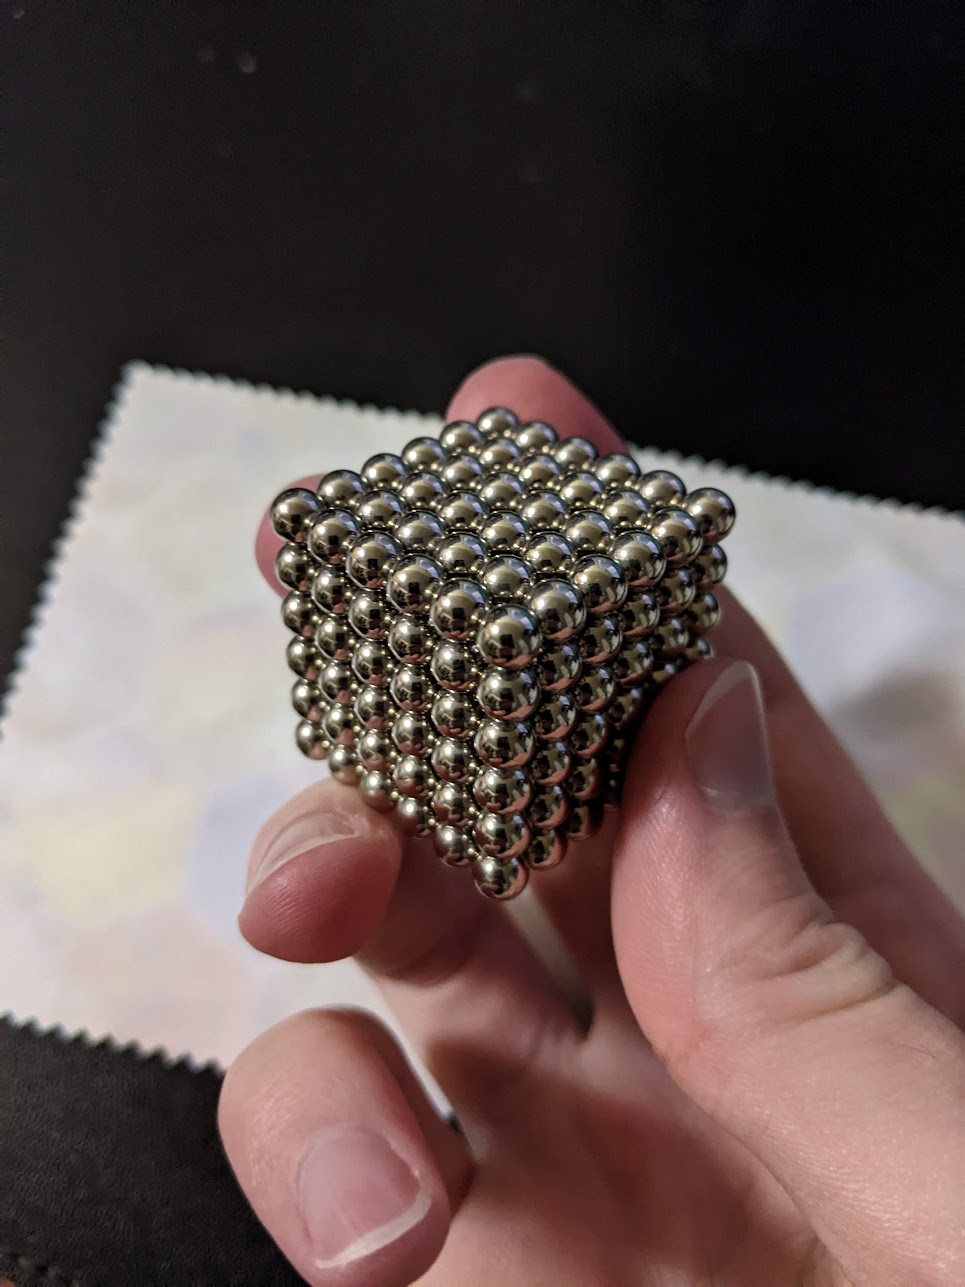
\includegraphics[width=150pt]{image1.jpg}
		\label{fig:image1}
		\caption{Cube of 256 Spheres}
	\end{figure}
	
	
	When the image of Figure 1 is provided, ChatGPT recognizes it as a configuration of metallic spheres in the shape of a cube. About 70\% of the time, it also infers correctly that the length of the side is 6, and arrives at $6^3=256$, the correct answer. A cube is probably the simplest 3d shape to reason about, and so it's not terribly surprising that ChatGPT can get this one correct. There is also perhaps some meta-knowledge the model possesses, in that magnetic spheres like the ones I use here are often sold in units of $256$ spheres, often displayed as cubes.
	\\
	
	\begin{figure}[h!]
		\centering
		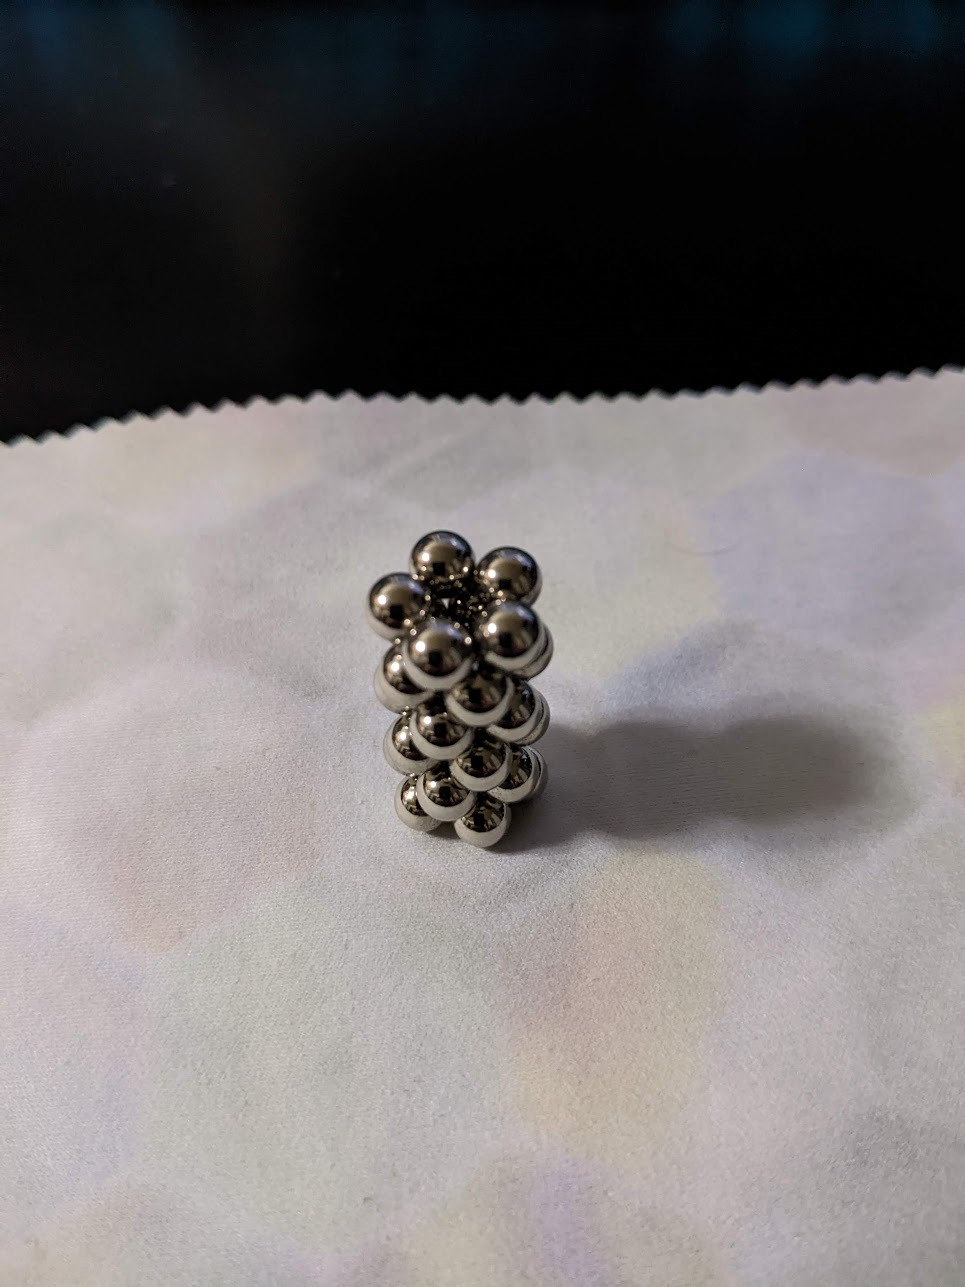
\includegraphics[width=150pt]{image2.jpg}
		\label{fig:image2}
		\caption{"Tube" of 30 Spheres}
	\end{figure}
	
	Figure 2 shows what I would describe as a stack of 6 pentagons, though the stacks are tightly nested so that the spheres aren't in "columns". The answer is obviously $5 \times 6 = 30$, but ChatGPT has a hard time assessing the structure. It's complete response is:
	\\
	
	\begin{lstlisting}
From the image, we can observe that the structure is a vertical stack of spheres forming a 3D configuration with a consistent repeating pattern. To determine the total number of spheres:

1. **Top layer:** There is 1 sphere.
2. **Second layer:** There are 6 spheres arranged in a hexagonal pattern.
3. **Third layer:** Again, there are 6 spheres in a similar hexagonal pattern.
4. **Bottom layer:** There appears to be a single sphere at the very base.

### Total number of spheres:
- Top layer: 1
- Second layer: 6
- Third layer: 6
- Bottom layer: 1

**Total = 1 + 6 + 6 + 1 = 14 spheres.**

Let me know if you'd like a different perspective or deeper analysis!
	\end{lstlisting}
	
	It's correct in that it is a vertical stack with a consistent pattern, but then tries to break it down into layers and gets it completely wrong. Even with multiple samples of prompting with this image, it's consistently wrong, and often guesses 14 or 25 spheres.
	\\
	
	\begin{figure}[h!]
		\centering
		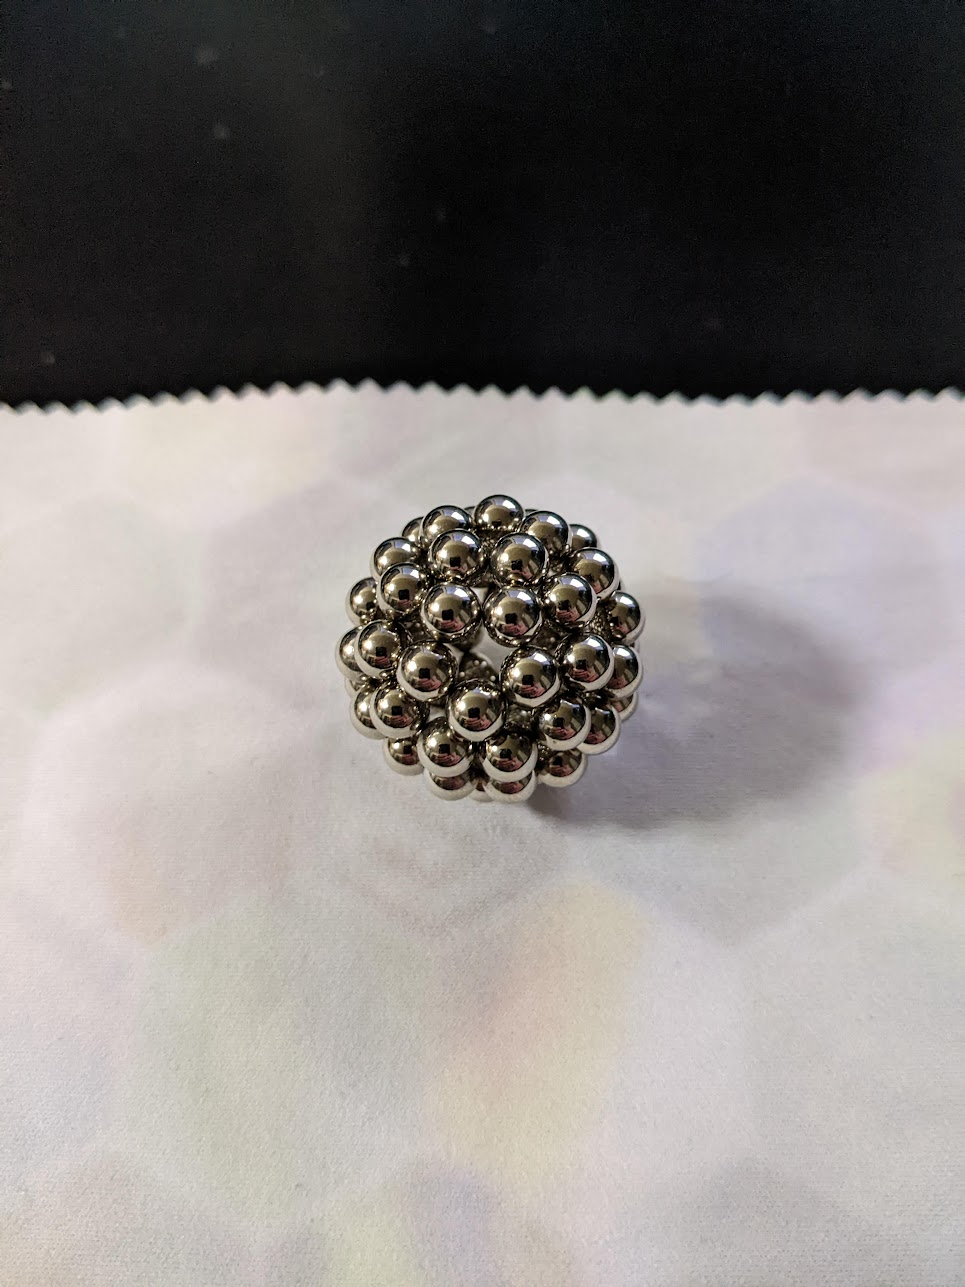
\includegraphics[width=150pt]{image3.jpg}
		\label{fig:image3}
		\caption{Dodecahedron of 60 Spheres}
	\end{figure}
	
	This last image of Figure 3 either depicts 12 pentagons arranged in a dodecahedron, or 20 triangles arranged in an icosahedron, depending on your perspective. In any case, the correct answer is $5 \times 12 = 3 \times 20 = 60$.
	\\
	
	This is empirically the most difficult for ChatGPT to assess. Even when analyzing the structure, often its best guess for shape is either some "symmetrical arrangement of spheres forming a 3D shape" or some "sphere-like cluster made of smaller metallic spheres, closely packed together". Despite the prompt asking for a clear answer, most of the time it doesn't give a number, as if it just gives up and is only willing to help me count it myself. Occasionally it suggests that the spheres are packed in some sort of triangular or tetrahedral number sequence, and uses a formula to conclude with a wrong answer.
	\\
	
	A sample response from ChatGPT for this one:
	\begin{lstlisting}
The structure in the image resembles a sphere built with a triangular or tetrahedral stacking pattern. In such configurations, the total number of spheres can be determined by summing the number of spheres in each layer.

For a tetrahedral stacking, the number of spheres in each layer increases according to triangular numbers:  
- Layer 1: 1 sphere  
- Layer 2: 3 spheres  
- Layer 3: 6 spheres  
- Layer 4: 10 spheres, and so on.

The total number of spheres in a tetrahedral arrangement of \( n \) layers is given by the formula:  
\[
T_n = \frac{n(n+1)(n+2)}{6}
\]

From the image, it seems to have 5 layers:
- Layer 1: \( 1 \) sphere  
- Layer 2: \( 3 \) spheres  
- Layer 3: \( 6 \) spheres  
- Layer 4: \( 10 \) spheres  
- Layer 5: \( 15 \) spheres  

Adding these:
\[
1 + 3 + 6 + 10 + 15 = 35
\]

Thus, there are **35 spheres** in total.
	\end{lstlisting}
	
	
	\section{Conclusion}
	
	ChatGPT failed the majority of the visual reasoning tasks I provided, excepting just the simple cube. My intuition for this consists of a few different thoughts. One is the limitations of image analysis and computer vision, particularly in an automated context like this where visual information can come from many bands and for many different sorts of tasks. Incorporating visual understanding for general-purpose instructional machines is a very large task.
	\\
	
	The second intuition for the struggling of this problem type is that it requires both spatial and mathematical reasoning. Gauging depth in the image, identifying spheres in a small sense, identifying structures/patterns in the arrangement of those spheres in a larger sense, and using mathematical reasoning of the identified structure to calculate the total number of spheres is a difficult task for a model not specifically fine-tuned for it.
	
	
\end{document}